%---------------- COMMENT FOR IMPORTING ----------------------
%\RequirePackage{lineno}				
%\documentclass[12pt]{report}		
%\pagestyle{headings}
%\input{ST-input2}							

%\setcounter{chapter}{0}
%\begin{document}								
%\setpagewiselinenumbers
%\linenumbers
%\tableofcontents
\graphicspath{{Appendix/figures_A/}} 
%-------------------------------------------------------------


\chapter{Methods for Background Subtraction}
\label{chap:ap_A}

This section introduces the notion of background subtraction, discusses the requirements of a good background model, describes three algorithms of interest and reviews the literature on these particular background subtraction algorithms.

When performing video analysis, often the first step is to segment the foreground from the background. In order to do this we must think of the foreground and background as two complementary sets. The specific definition of foreground can vary between applications, but generally foreground is defined to be the moving objects of interest in a video sequence and the background is defined to be everything else. Often, more information is known about the background as it tends to vary less than the foreground. For example a surveillance camera located in a supermarket will often show a background scene where there is no activity. This allows the user to gain lots of information about the background, and so interest is directed at the foreground. Once accurate segmentation has been performed, later stages may consist of attempting to track a particular object or classify the scene as a particular event so the importance of correct segmentation is evident. Whilst a number of methods for segmentation exist, background subtraction is by far the most popular, mainly due to its computational efficiency. Although many algorithms for background subtraction have been discussed in the literature such as in \cite{sen2004robust}, the topic is still far from complete, and is of great interest to researchers. 

%\begin{figure}[h]
%  \centering
%  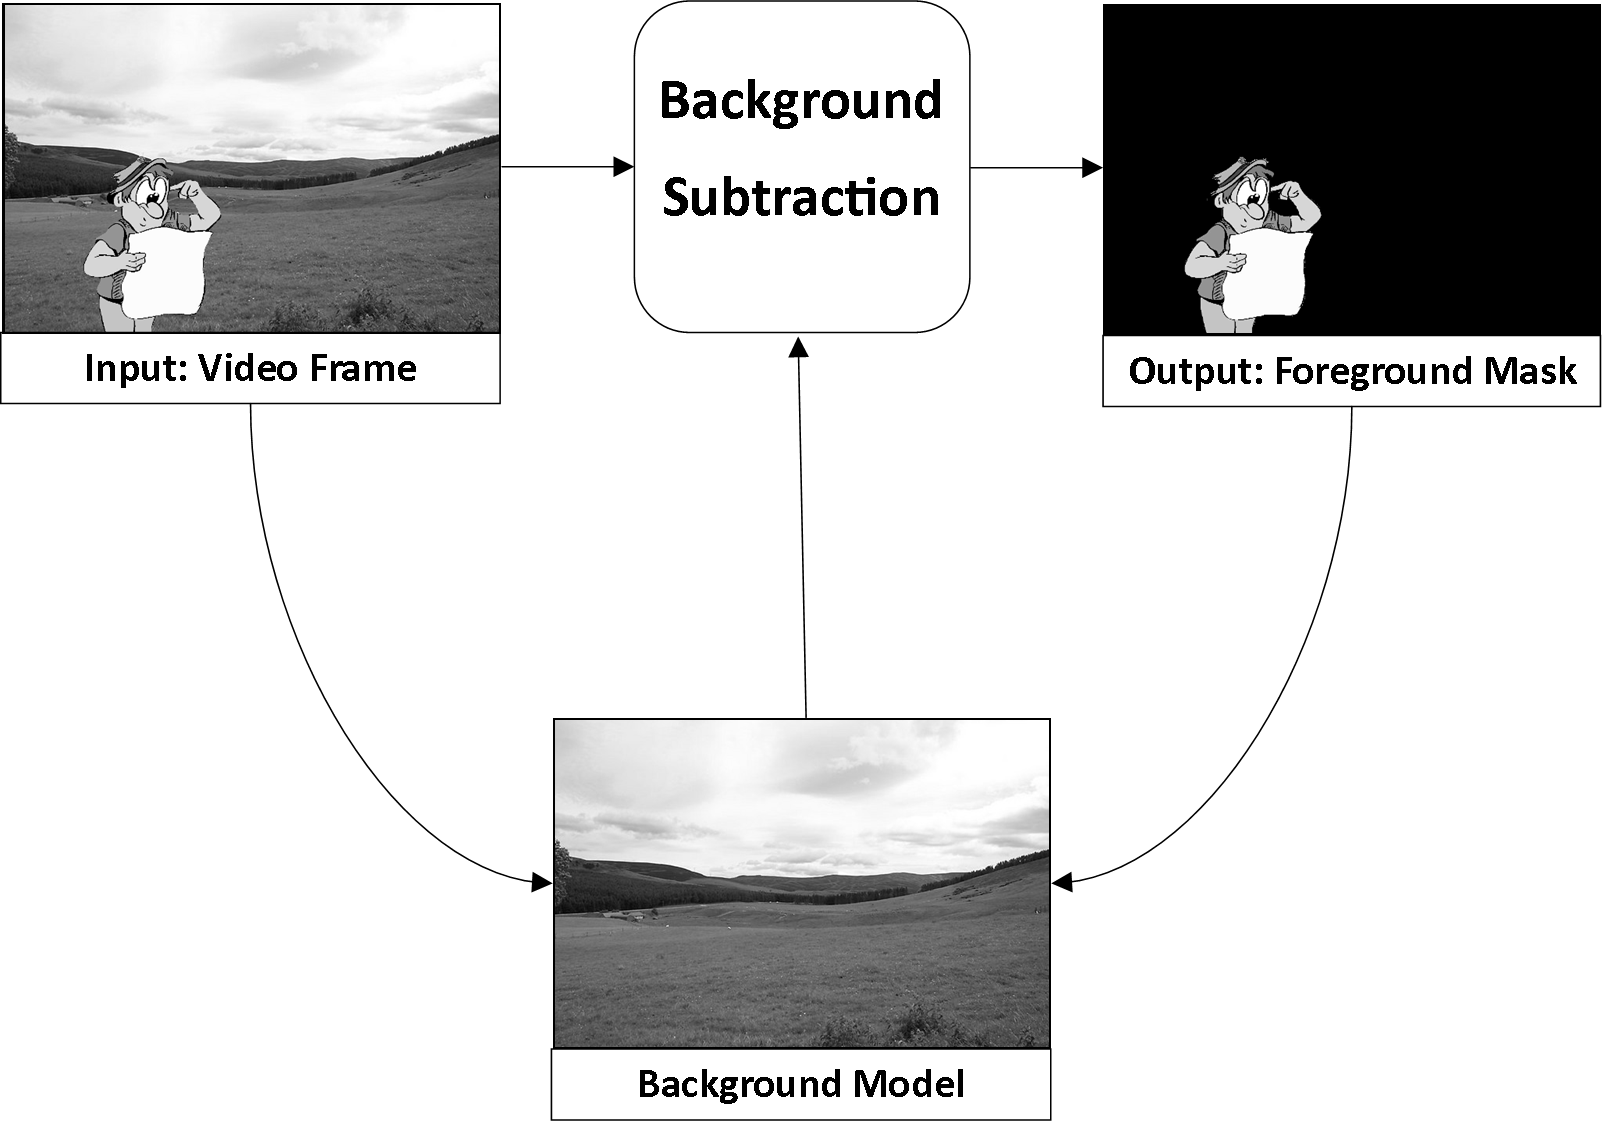
\includegraphics[width = 14cm]{backgroundsubtraction}
%  \caption{The background subtraction process}
%  \label{fig:bgs}
%\end{figure}

The basic idea behind background subtraction is that a model of the background is created and then this background model is subtracted from each video frame in turn; what remains is classified as the foreground. According to \cite{parks2008evaluation}, background subtraction is made up of four processes; preprocessing, background modelling, foreground detection and post processing. Firstly, the video needs to be prepared for analysis this is known as pre-processing. The video is split up into frames, the frame size and rate are often reduced in order to save memory and computational effort. It is also common for the video to be converted from colour to grayscale, as analysis in grayscale is computationally lighter than colour analysis. For each video frame, a matrix of grayscale pixel intensity is stored. The grayscale mapping can be seen in Figure \ref{fig:grayscale}, where 0 refers to black, and 255 indicates a white pixel. Using this luminance pixel intensity, information can be stored about the image in matrix form. For the remainder of this dissertation, $I_t(x,y)$ refers to as the intensity of pixel in position $(x,y)$ and $\pmb{I}_t$ represents the entire frame of pixel intensities at time $t$. The background estimate is represented by $\pmb{B}_t$ for the whole frame and ${B_t(x,y)}$ for the background estimate for pixel $(x,y)$ at time $t$. 

\begin{figure}[h]
  \centering
  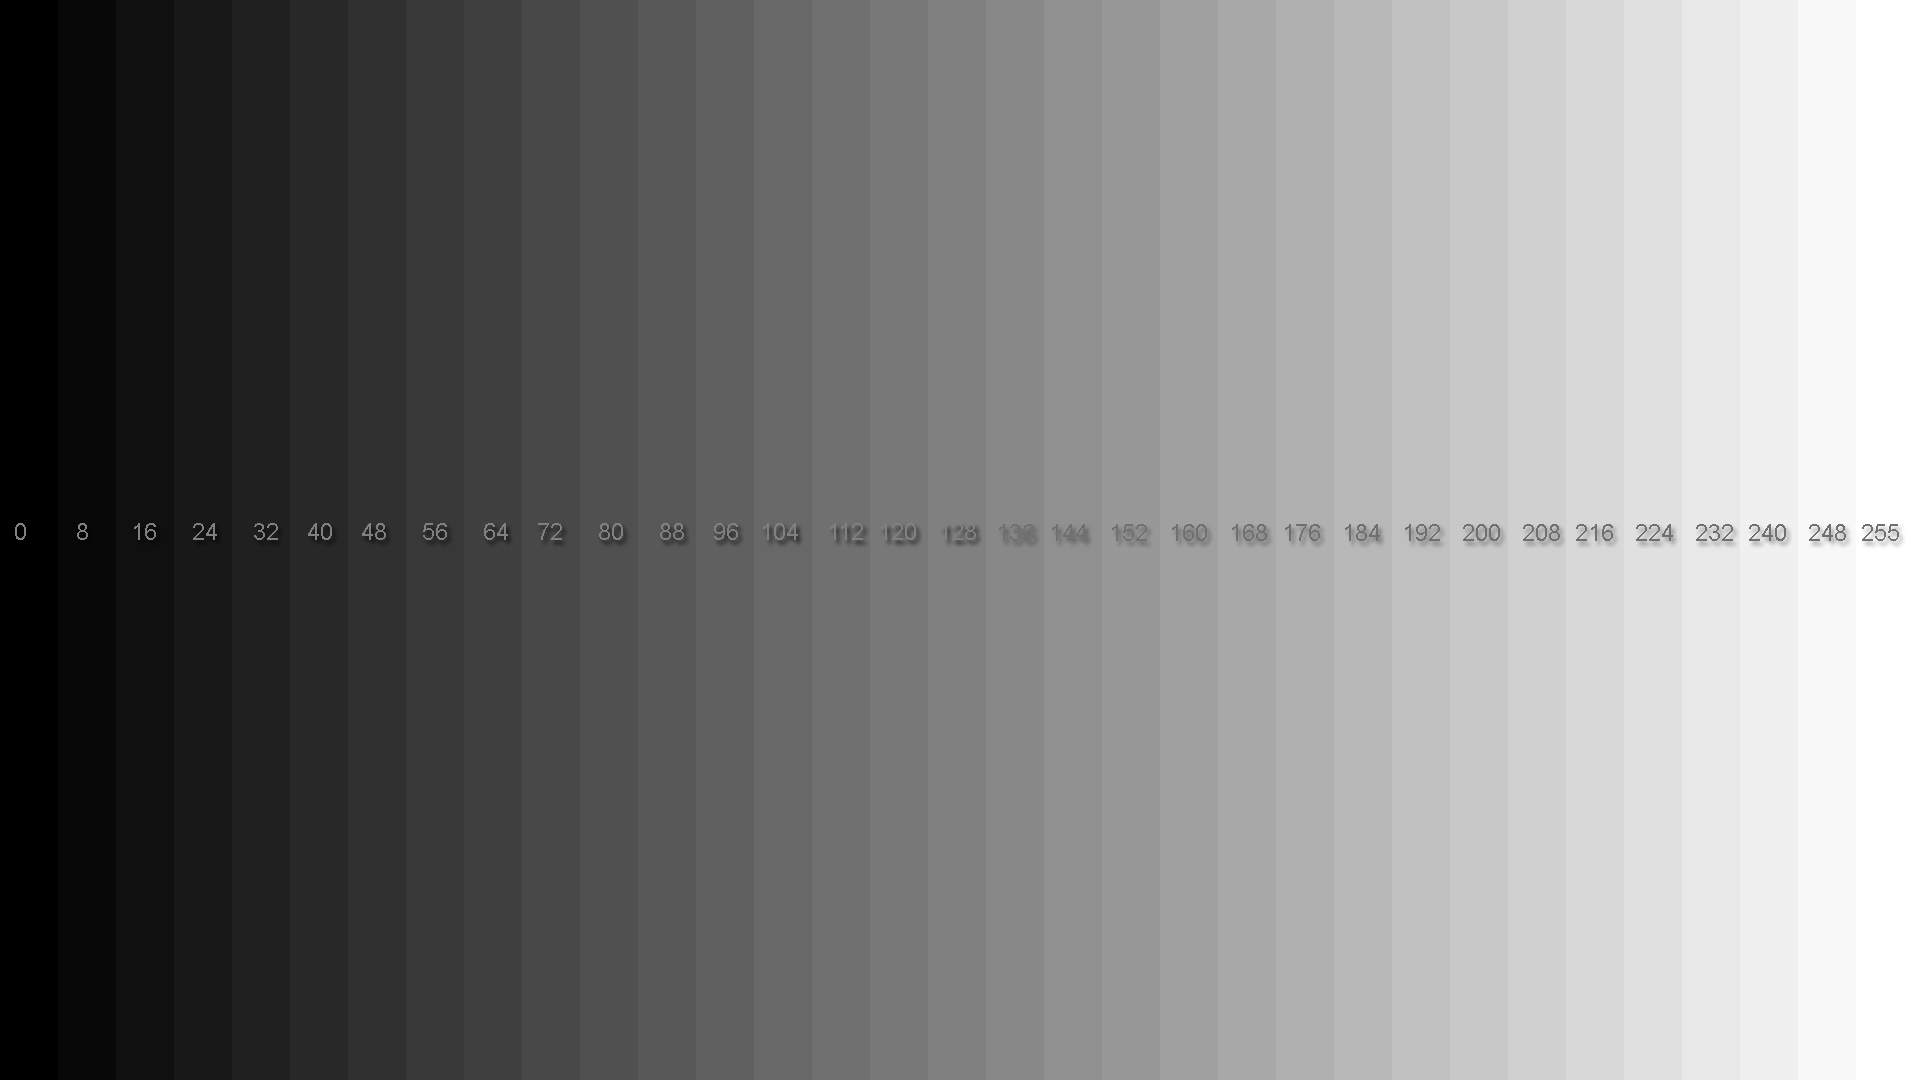
\includegraphics[width = 8cm]{grayscale.JPG}
  \caption{The grayscale luminance scale. A black pixel is represented by 0 and a white pixel is represented by 255.}
  \label{fig:grayscale}
\end{figure}


\section{Background Modelling}
\label{sec:background-modelling}
A background model is simply an estimated image of the background that does not contain any objects of interest. Figure \ref{fig:bg} visualises what a background model may look like when calculated for a busy traffic scene. The images have been using created from a video collected by \cite{benton2008background} and an adaption of his code which can be found in his excellent article on methods for background subtraction.   

\begin{figure}[h]
  \centering
  \begin{subfigure}[b]{0.4\textwidth}
                \centering
                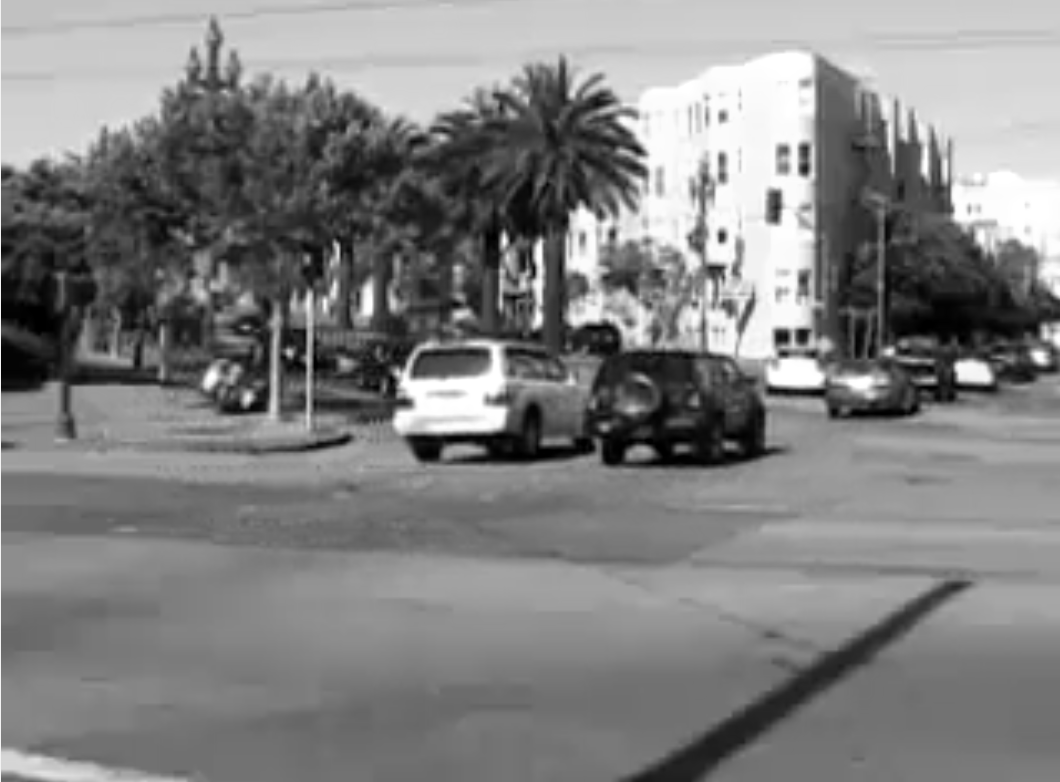
\includegraphics[width=\textwidth]{sethactual}
                \caption{Original frame.}
                \label{fig:bgbw}
        \end{subfigure}
\quad
\begin{subfigure}[b]{0.4\textwidth}
                \centering
                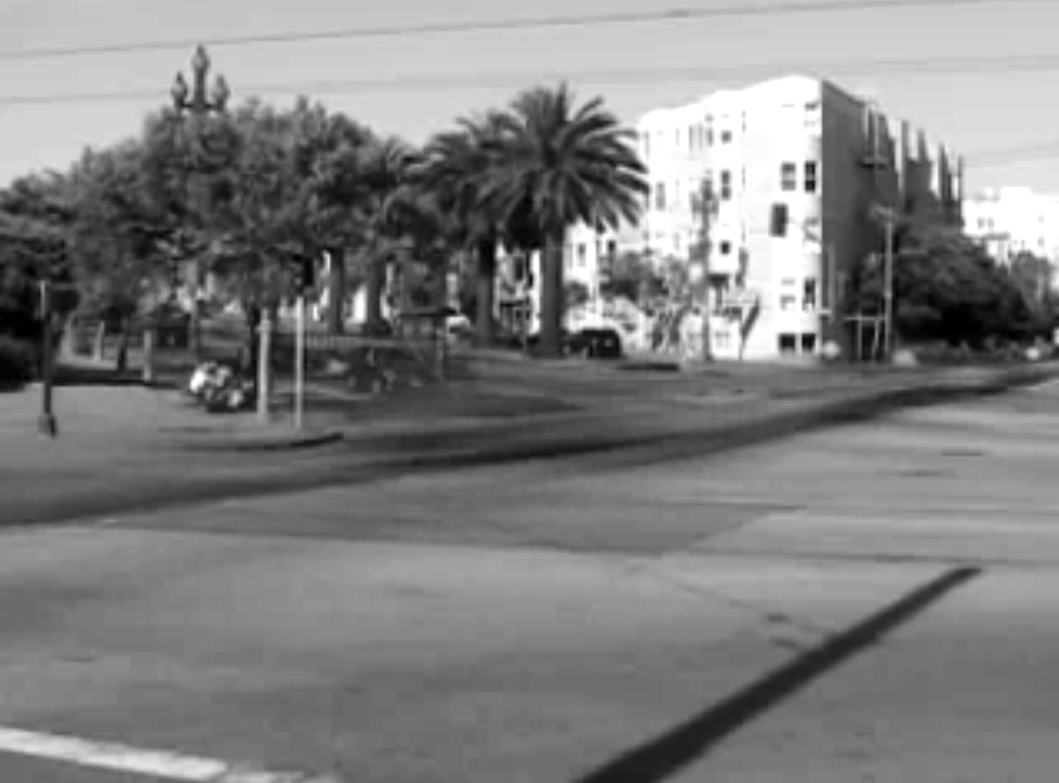
\includegraphics[width=\textwidth]{sethbgm}
                \caption{Estimated background.}
                \label{fig:bgbg}
        \end{subfigure}
\caption{A frame of a busy traffic scene and the background model of the scene as estimated using the Approximate Median method as discussed in Section \ref{sec:approximate-median}. Video and code adapted from \cite{benton2008background}. \label{fig:bg}}
\end{figure}

Although a static background could be used for short indoor sequences, most real-world video sequences require a dynamic background model. \cite{piccardi2004background} suggests that a background model should be able to adapt to deal with illumination changes, high frequency repetitive background objects and changes in background geometry. 

Illumination changes can be separated into gradual changes, or rapid changes. Gradual changes in illumination are mainly due to the light changing throughout the day. Rapid changes in illumination may occur when clouds cover the sun in outdoor scenes or a light being switched on or off in interior scenes.

High frequency background objects are mainly found in outdoor footage such as leaves waving in the wind, water rippling or rainy weather. These small movements are actually part of the background so care should be taken to use an algorithm which detects them as such. Examples may also occur indoors but these are often less prominent.

Changes in background geometry refers to when an object in the background is moved, this means that the object should change from being part of the background model to a foreground object of interest, and then back to being back of the background when it becomes stationary. In order for good segmentation we wish this process to be as smooth and fast as possible. Examples of this are very common in real videos, such as a chair being repositioned in a room such as in \cite{toyama1999wallflower} or a car driving into a car park as foreground, and then parking therefore becoming part of the background as can be seen in \cite{pets2001}.

\cite{barnich2011vibe} discuss the importance for background models to be able to deal with bootstrapping. They need to be able to initiate an accurate background model in the absence of a complete and static training set. This is a common problem, particularly in surveillance videos in busy areas such as a supermarkets and airports. The scene may constantly have objects in the foreground and so maintaining an accurate background model may be difficult. 

However, the most important requirement for a background model is that it is computationally inexpensive and has low memory requirements. This is always a major issue when comparing models if it is necessary to work in real-time as many applications demand.

 The Wallflower data set collected by \cite{toyama1999wallflower} is a useful data set of seven short video sequences in the public domain which are often used to test the capabilities of background subtraction methods as each of the video sequences represents a different, potentially problematic scenario for background maintenance. A number of papers have used this data set and so it is becoming a useful standard for comparison of results. In fact, \cite{bouwmans2011recent} strongly recommends all researchers to use this set as a base for future experiments. It is for these reasons that the Wallflower data set is used in this dissertation to compare background subtraction techniques. 

\section{ Foreground Detection}
\label{sec:techn-backgr-subtr}
It is possible to separate algorithms for background subtraction in terms of pixel based methods and region based methods. The latter may seem more intuitive as one expects foreground to be in clusters and not exist as isolated pixels. Neighbouring pixels obviously have some impact on whether the pixel is foreground or background, and region based techniques such as  \cite{elgammal2000non} and \cite{toyama1999wallflower} use this knowledge to segment the images into regions and then create a background model based on these regions. However, there is one big downside to region based techniques which is that they are often a lot more complex to run then pixel based techniques. Pixel based methods assume that the pixels observed are classified as foreground independently of each other. As computational efficiency is of primary importance, only pixel based techniques are considered in this dissertation. 

It is also possible to categorise these algorithms as recursive and non-recursive. A non-recursive algorithm maintains a buffer or window of N previous video frames and estimates a background model based on the statistical properties of these frames. This constantly moving buffer often needs to be fairly large in order to obtain accurate results, and therefore can quickly become computationally heavy. Recursive techniques update the background subtraction every time a new frame is stored so has no need to buffer previous frames. This dissertation considers both of these types of algorithm.

\subsection{Frame Difference (FD)}
\label{sec:frame-difference}

This non recursive frame difference method is arguably the simplest method of background subtraction and is computationally inexpensive to run. The basic idea of frame difference is to assume that for each frame the previous frame is the background model. This is the same as having a buffer of one frame. The background model is compared with the current frame, pixel by pixel. The criterion which determines whether pixel $I_t(x,y)$ is belongs to the background or foreground is given in equation (\ref{eqn:ff}).
%
\begin{equation}
  |I_t(x,y) - I_{t-1}(x,y)| > \tau.
\label{eqn:ff}
\end{equation}
%
 If the intensity of pixel $(x,y)$ in the the $t^{th}$ frame  $I_t(x,y)$, is significantly different to the intensity of pixel $(x,y)$ in the ${t-1}^{th}$ frame $I_{t-1}(x,y)$, then the pixel is classified as foreground, otherwise it is classified as background. The output of this method is strongly dependent on the threshold $\tau$. If $\tau$ is too large then only drastic changes in pixel intensity will be classified as foreground, whilst if $\tau$ is too small then any slight change in pixel intensity will be classified as foreground. The challenge of picking a good threshold is not a challenge restricted to frame differencing methods and is something that is encountered in the other background subtraction methods to be discussed. 

The two main advantages to using this method are that it is computationally light and it has highly adaptive background model. The background model is so adaptive because it is solely based on the previous frame $\pmb{I}_{t-1}$. This means that the model can deal with small repetitive movements in the background such as trees moving in the wind.

The disadvantages that arise when using the frame differencing method are overreacting and the aperture problem. Due to frame differencing having a highly adaptive background model, it can overreact when an object becomes stationary for a very short amount of time and classify a pixel as background when actually it is a slow moving part of the foreground. So a if a pedestrian stands still for a few frames, they will seemingly disappear from the foreground. This downfall is due to the buffer size of one frame which is used, with the severity of the problem will depend on the frame rate as compared to the speed of the foreground. If the frame rate is much faster than the movement of the foreground, the foreground will be seem to be stationary between certain frames, but if the frame rate is much slower, the foreground will seem to jump around and will not be smooth. 

The aperture problem occurs when objects partially exhibit uniformly distributed pixel intensity. To illustrate the aperture problem with uniformly distributed pixels consider the example of observing a moving car. The interior pixels of the side of a car are classified as the background and only the outline is classified as foreground as can be seen in Figure \ref{fig:carff}. White pixels indicate foreground and black represents the background as detected by the frame differencing algorithm. There is a large patch of black in the centre of the car, and so the frame method has incorrectly classified a large part of the car as background. 

\begin{figure}[h]
  \centering
  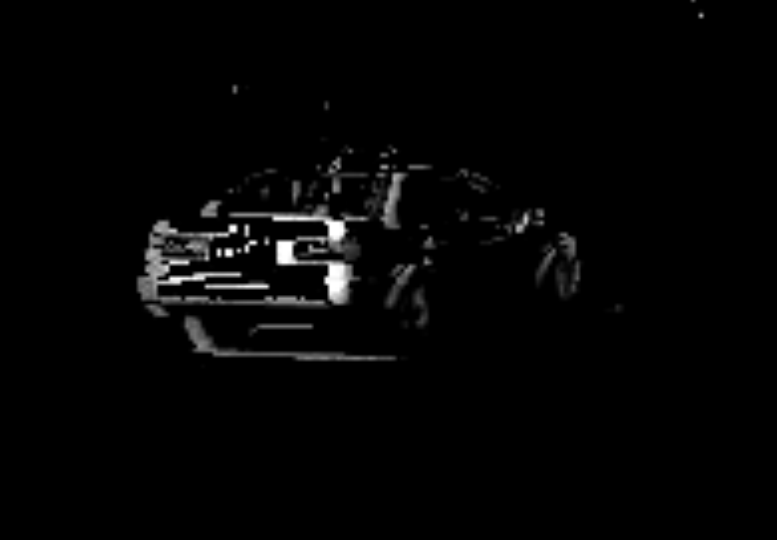
\includegraphics[width = 7cm]{carff.png}
  \caption{A moving car as detected by the frame differencing method. The white pixels represent foreground and the black ones represent background. Although the outline has been well detected, the middle of the car has been incorrectly classified as background due to the highly adaptive background model used in frame differencing.}
  \label{fig:carff}
\end{figure}

Although frame differencing is a fast algorithm, its highly adapting background causes issues with efficiency of the algorithm. The approximate median filter is now considered, which uses N buffer frames instead of just one as in frame differencing.


\subsection{Approximate Median Filtering (AMF)}
\label{sec:approximate-median}

Approximate median filtering is a more advanced version of the median filter algorithm. In median filtering, N frames are buffered and the background model $\pmb{B}_t$ is calculated as the median of the previous N frames. Although was found to be a fairly robust non-recursive method in \cite{gloyer1995video}, constantly retaining a large frame buffer meant large memory requirements computationally. An improvement to this method was proposed in \cite{mcfarlane1995segmentation}. They devised a recursive method entitled approximate median filtering which uses equation \eqref{eq:5} 
%
\begin{eqnarray}
  \label{eq:5}
  \mbox{If } I_t(x,y)  >  B_t(x,y) & \Rightarrow& B_t(x,y) = B_t(x,y) + 1 \nonumber, \\
\mbox{If } I_t(x,y)  <  B_t(x,y) & \Rightarrow& B_t(x,y) = B_t(x,y) - 1 .
\end{eqnarray}
%
to maintain the background model.

If the value of a pixel in the current frame $I_t(x,y)$ has a value larger than the corresponding background pixel $B_t(x,y)$, update the background estimate by adding one. 
If the pixel $I_t(x,y)$ has a value smaller than the corresponding background pixel $B_t(x,y)$, update by removing one. The background estimate will eventually converge to an estimate where half of the input pixels are greater than the background and half are less, although the speed at which this converges depends on the frame rate. This method offers a good compromise as it can perform well whilst remaining computationally light. This is an example of a more slowly adapting background model compared to frame differencing, which means that it can incorporate a longer visual history, without the computational cost of a large buffer such as in median filtering.

\subsection{Mixture of Gaussians (MoG)}
\label{sec:mixt-gauss-mog}
This method has enjoyed much popularity since its proposal in \cite{friedman1997image}. Mixture of Gaussians (MoG) works by modelling the pixel intensity values over time with a weighted mixture of Gaussians. Unlike frame differencing and approximate median methods, the background model is now parametric and not based on a single estimated background matrix $\pmb{B}_t$. There is no need to store a buffer of frames in MoG as the parameters are updated on line at each stage and so this is classed as a recursive method. 

The pixel intensity distribution $f(I_t(x,y) = u)$ is modelled  as a mixture of $K$ Gaussians, or written mathematically,
%
\begin{equation}
  \label{eq:24}
  f(I_t(x,y) = u) = \sum_{i=1}^K \omega_{i,t} \quad N(u; \mu_{i,t}, \sigma_{i,t}^2).
\end{equation}
%
Typically $K$ ranges from $3 - 5$ depending on the demands of the video and the storage availability. In equation \eqref{eq:24}, $\omega_{i,t}$ is a weight representing the portion of data accounted for by the $i^{th}$ component and $N (u;\mu_{i,t}, \sigma_{i,t})$ is the $i^{th}$ Gaussian component with intensity mean $\mu_{i,t}$ and standard deviation $\sigma_{i,t}$.

For input pixel $I_t(x,y)$, we must identify the component $i$ which is closest to $I_t(x,y)$.

\begin{definition}
The $\hat{i}^{th}$ component is considered to be the matched component for $I_t(x,y)$ if
\begin{equation}
  \label{eq:6}
  |I_t(x,y) - \mu_{\hat{i},t-1}| \leq D \sigma_{\hat{i},t-1},
\end{equation}
where $D$ defines a small positive deviation threshold. 
\end{definition}
Once a matched component $\hat{i}$ has been chosen for pixel $I_t(x,y)$, one then needs to update the relevant Gaussian parameters as shown in equation \eqref{eq:27}.

\begin{eqnarray}
  \label{eq:27}
\mu_{\hat{i},t } =& (1-\rho)\mu_{\hat{i},t-1} +& \rho I_t(x,y), \\
\sigma^2_{\hat{i},t} =& (1-\rho)\sigma^2_{\hat{i},t-1} +& \rho(I_t(x,y) - \mu_{\hat{i},t})^2.
\end{eqnarray}

This Gaussian mixture method uses a learning parameter $\rho$ to update the Gaussian parameter. The choice of $\rho$ will affect how quickly the Gaussian adapts to changes in the background and foreground. For example if $\rho$ is large, more weight is given to the new pixel, whilst if $\rho$ is small, less weight is given to the new value. 

At each time step, the weights are also updated with the following equation 
%
\begin{equation}
  \label{eq:28}
  (1-\alpha) \omega_{\hat{i},t-1} + \alpha.
\end{equation}
%
where $\alpha$ refers to the learning rate which is constricted by $0 \leq \alpha \leq 1$. The relationship between  $\rho$ and $\alpha$ is given by
%
\begin{equation}
  \label{eq:29}
  \rho \approx \frac{\alpha}{\omega_{\hat{i},t}}.
\end{equation}
%
There are occasions where a matched component cannot be found, in this case the component with the least weight is replaced by a new component with mean $I_t(x,y)$, large initial variance $\sigma_0$ and small weight $\omega_0$. This replacement system allows infrequent Gaussian components to be replaced with more up to date components, allowing the mixture of Gaussians methods to adapt freely to change. The rest of the components are then calculated recursively as so,
%
\begin{equation}
  \label{eq:210}
  \omega_{i,t} = (1-\alpha) \omega_{i,t-1}.
\end{equation}
%
in order to adapt to the newly defined component. Finally, all the weights are renormalised so that they sum to one.

To determine whether $I_t(x,y)$ is a foreground pixel, all the coefficients are first ranked by calculating the rank factor according to 
%
 \begin{equation}
   \label{eq:212}
   \frac{\omega_{i,t}}{\sigma_{i,t}}.
 \end{equation}
%
High-ranking components thus have low variance and high probabilities, which are typical characteristics of background pixels. If $i_1, i_2, \ldots, i_K$ is the component order post-sorting, the first $M$ components that satisfy the following criterion, 
%
   \begin{equation}
     \label{eq:211}
     \sum_{k=i_1}^{i_M}\omega_{k,t} \geq \Gamma,
   \end{equation}
%
are declared to be background components. This criterion effectively ensures that the components that are most likely to be background components are classified correctly, according to the weight threshold $\Gamma$. This $\Gamma$ ensures that the weights $\omega_{k,t}$ are large enough, as otherwise, components with average weights but very small variances would be classed as background, possibly incorrectly. 

A pixel $I_t(x,y)$ is classed as a foreground pixel if $I_t(x,y)$ is within $D$ times the standard deviation from the mean of any one of the background components. 

The MoG method uses the strong assumption that the background is more frequently visible than the foreground and that the background has significantly lower variance which cannot always be held to be true in all frames of a video. If the foreground takes up most of the screen for a large number of frames and the foreground pixels have low variance (such as a plain jumper) this is called the camouflage problem and will be considered further in Section \ref{sec:implementation}.The MoG method is generally good at suppressing background noise but not very adaptive to rapid illumination. This is especially true if a scene has been similar for a long time which is common in surveillance data, because the Gaussian variance components become very small.

%The performance of these three algorithms in the literature is discussed in Section \ref{sec:literature-review}. 


% \section{Discussion of Current Methods}
% \label{sec:literature-review}

% There have been a number of informative surveys written about background subtraction techniques over the years which reflects the continually growing interest in this subject. Notable studies are \cite{cheung2004robust}, \cite{piccardi2004background} and \cite{bouwmans2011recent}.

% \cite{cheung2004robust} is an excellent survey paper that applies the frame differencing, approximate median and mixture of gaussian algorithms to an urban traffic scenario. This setting involves both pedestrian and vehicle traffic and they considered four different scenarios which were a bright day, a foggy day, a snowy day and a busy day. By studying these different scenarios the algorithms could be tested on adaption to illumination during the bright scene, high frequency repetitions such as snow and rain, and bootstrapping on the busy day. Results showed that MoG experienced the best performance overall but it required a lot of tuning and was very sensitive to global illumination changes. They found that all of the algorithms tested suffered in the noisy rain and snow scenarios, but frame difference performed significantly worse than the other methods throughout. Approximate median seemed to be a good compromise as it only performed slightly worse than MoG, and has the benefit of a huge improvement in computational efficiency. 

% %Piccardi investigation into computational complexity, but unfortunately no experimental results. (\cite{piccardi2004background} EXPAND

% A more recent survey of background subtraction algorithms has been carried out in \cite{bouwmans2011recent} which in particular considers the many improvements that have been suggested to the mixture of gaussians algorithm over the years. These improvements are tested on the Wallflower test set and the findings indicate that the adjustments generally improve the accuracy on all seven video sequences over the original algorithm, although sometime at the cost of computational expense. The paper is quite critical of the basic mixture of Gaussians, arguing that backgrounds with fast variations cannot be modelled accurately with only 3-5 Gaussians.

% \cite{benton2008background} compares all three algorithms on a real-life traffic intersection scene like \cite{cheung2004robust}. Although the article does not quantify results, it compares the algorithms visually and seems to indicate that approximate median performs very well given the computational efficiency, a similar result as seen in the Cheung paper.

% \cite{parks2008evaluation} offers a good evaluation of a number of algorithms, including slight variations of the three aforementioned. The algorithms have all been adapted to be able to compute colour processing on thirteen video sequences. They also compare an adaptive Gaussian mixture model (AGMM) which is a variant on MoG which was proposed by \cite{zivkovic2006efficient} which automatically adapts the number of gaussians used to model pixels. They compared algorithms on the wallflower data set using standard metrics and found approximate median filtering performed best when efficiency was taken into account but discussed the limitation that you cannot model the variance of a pixel with AMF. The AGMM extension did not improve performance over MoG but it did make the algorithm quicker to run and more memory efficient, and this algorithm was recommended if a fair amount of computational power is available. 

% \cite{lin2009learning} discuss background modelling in terms of representation, initialisation and maintenance and claims that the initialisation aspect has been neglected in the literature. Most of the popular methods for background subtraction only use a simple initialisation as they are fast to adapt. This fast adaption means that the importance of the initialisation frame decreases quickly. 

% \cite{bhaskar2010video} show that heavy tail distributions can model the foreground and background in a better way than the Gaussian distribution. The paper argues that a method based on the Cauchy distribution might be more applicable as the heavy tails of the distribution could make the algorithm more adaptive to the dynamic changes of background scenes. Also as the Cauchy distribution does not involve exponential operations, it is argued that is might be more computationally efficient than MoG. The question of if natural image analysis suit Gaussian methods is discussed in \cite{srivastava2003advances} and this debate of which distribution is most suitable when modelling pixel intensities of natural images could be interesting to investigate further.

% One disagreement which seems to arise frequently in the literature is whether colour or grayscale analysis should be used. \cite{cheung2004robust} decide to just use grayscale luminance methods for speed but a number of papers such as argue that using colour videos can aid performance, especially where images have low contrast. Colour can be useful when trying to distinguish between the actual moving foreground and the object's shadow. This type of ghost is often found even the very good background modelling methods. \cite{parks2008evaluation} seems to think that the significant increase in complexity required for colour based methods is a good trade off for the improvement in accuracy of algorithms, this is again another area that could be interesting to study further.  

% Most these papers suffer from the challenge of making a good threshold choice. Often a suitable threshold is calculated experimentally which is not ideal as it can be quite time consuming. \cite{parks2008evaluation} stress the benefits of having some sort of rough idea of a good threshold. Perhaps a heuristic technique could be standardised to aid the initial choice of threshold. It could also be useful if the threshold was dependent on the spatial location of the pixel of interest $(x,y)$, so that the threshold could be lower in areas of low contrast and higher in areas of high contrast. This possibility is discussed as part of blob tracking in \cite{fuentes2003tracking}.

% The approximate median filter seems to have been found to be good across the board as it gives a robust performance considering its low implementation. Mixture of Gaussian has proved to be popular throughout the literature but it seems there are real concerns about its efficiency. The AGMM adaption and others discussed in \cite{bouwmans2011recent} seem to offer improvements and if efficiency is not a problem the mixture of gaussian type algorithms are recommended as a good algorithm of choice.  


% \section{Quantitative Analysis}
% \label{sec:quant-analys}

% A quantitative way to characterise the accuracy of detection algorithms is to use three performance metrics; recall; precision and percentage of correct classifications (PCC). These measures calculate how accurate the segmentation is for a particular frame by comparing the estimated foreground and background with the true values. These true values are calculated by segmenting a frame by hand, this frame is known as the ground truth. Figure \ref{fig:gt} shows the original frame and ground truth for a still from the Wallflower data set Waving Trees taken from \cite{toyama1999wallflower}.

% \begin{figure}[h]
%   \centering
%   \begin{subfigure}[b]{0.4\textwidth}
%                 \centering
%                 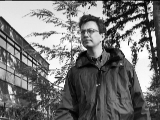
\includegraphics[width=\textwidth]{wtbw}
%                 \caption{Original frame}
%         \end{subfigure}
% \quad
% \begin{subfigure}[b]{0.4\textwidth}
%                 \centering
%                 
\includegraphics[width=\textwidth]{wtgt}
%                 \caption{Ground truth}
%                 \label{fig:wtgt}
%         \end{subfigure}
% \caption{A frame from the Wallflower Waving Trees data set and the corresponding hand segmented ground truth frame to be used as a comparison. In the ground truth frame white corresponds to foreground and black represents background.}\label{fig:gt}
% \end{figure}

% In order to quantify how well an algorithm is working, we must consider Type I errors and Type II errors. A Type I error is a false positive (FP), this is experienced when the algorithm classifies a pixel as foreground incorrectly. A Type II error is a false negative (FN), this where the algorithm has neglected to classify a foreground pixel correctly. If the algorithm works perfectly we will only have True Positives (TP) and True Negatives (TP).

% \begin{definition}
%   \label{def:1}
%   Recall is defined as the fraction of correctly identified foreground pixels over the number of ground truth foreground pixels which can be written mathematically as
% \begin{equation}
%   \label{eq:1}
% \text{Recall} = \frac{TP}{TP + FN}. 
% \end{equation}
% \end{definition}

% Recall is described to be the fraction of correct classification that are collected, so in background subtraction, this can be viewed as the the percentage of correctly identified pixels. Recall is always between 0 and 1. A value close to 1 implies high recall which means that all of the foreground pixels were correctly identified by the background subtraction algorithm. Recall cannot be used alone as a metric, as even if all of the foreground pixels are correctly detected, this does not give any information on about whether extra pixels have been misclassified as foreground. Hence precision is also used to quantify how accurate the algorithm is.

% \begin{definition}
%   \label{def:2}
%   Precision is defined to be the fraction of correctly identified foreground pixels over the number of detected foreground pixels in total, or when written mathematically
% \begin{equation}
%   \label{eq:2}
% \text{Precision} = \frac{TP}{TP + FP}.
% \end{equation} 
% \end{definition}

% This metric is also between 0 and 1, and a high precision value implies that of all the pixels classified as foreground, they are also foreground in the ground truth. We can not be sure if we have missed some foreground elements until we consider recall.

% If we wish to rank algorithms in order, it is useful to have one overall measure of the algorithms accuracy. A popular choice in the literature is percentage of correct classifications (PCC). 
% \begin{definition}
%   \label{def:3}
%   Percent of correct classifications (PCC) is defined to be 
% \begin{equation}
%   \label{eq:3}
%  \frac{TP+TN}{TP + TN + FP + FN},
% \end{equation}
% where TP, TN, FP and FN are defined as above. 
% \end{definition}

% Although PCC can be useful for ranking performance, it is important to not just rely on one metric. It is possible for a background subtraction technique to fail to detect any foreground in the test frame giving a recall value of 0, but the PCC could still be very high if the algorithm correctly identifies all of the true negatives. This is a good example of why metrics cannot be solely relied on, and reinforces the importance of visually analysing the output as well as considering metrics.


% \section{Implementation}
% \label{sec:implementation}

% Frame differencing and the approximate median filter are now implemented on the Wallflower data set. This data set was first created for use in \cite{toyama1999wallflower}. This data set was chosen as each video presents a particular challenge for the background subtraction algorithms. A brief description of the seven videos included in the  Wallflower data set follows.

% \begin{description}
% \item[Moved Object.]This video tests the ability of the algorithms to adapt to a change in geometry of the background scene. A person enters the room, moves the telephone and a chair and then leaves. The evaluation image is taken shortly after the person has left the room and we expect to see no foreground calculated by the algorithms.
% \item[Time of Day.]The focus in this video is to test how the algorithms can cope with gradual illumination changes. This change is supposed to imitate sunlight changing throughout the day but it is created manually inside which makes this video clip slightly unrealistic.
% \item[Light switch.]A light is switch on, and later switched off, the evaluation image is a few frames after the light has been turned off. This tests the algorithms ability to deal with rapid illumination changes. 
% \item[Waving Trees.]This video is designed to determine how well an algorithm can filter out high frequency oscillations in the background, which is here represented by a tree swaying in the wind. The challenge here is to correctly identify a walking man as foreground against the dynamic background.
% \item[Camouflage.]A person walks in front of a monitor and stands close to the camera so that he takes up most of the frame. The person's clothes are of similar intensity as the computer in the background, which can make segmentation more difficult.
% \item[Bootstrapping.]There is no clear background scene in this busy cafeteria sequence which makes a background model more difficult to maintain accurately. 
% \item[Foreground Aperture.]A person is asleep on a desk and wakes up half way through the video. The sudden appearance of foreground tests the algorithms ability to adapt to changes in the background quickly. 
% \end{description}

% The frame differencing method and the approximate median filter were implemented on all videos in the data set, and a threshold of 25 was chosen for both. For each video sequence, the ground truth is provided for one image which occurs just after a difficult stage of the video. Table \ref{tab:gt} represents displays the ground truths for each video and the evaluation of the foreground as calculated by each of the algorithms. 

% \begin{table}[ht!]
% \caption{Comparison of ground truth and evaluation images.}
% \centering
% \begin{tabular}{cccc}
% & Ground Truth & Frame Difference & Approximate Median\\
% \parbox[top]{30mm}{Moved Object} & 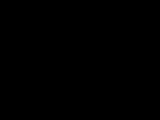
\includegraphics[width=30mm]{MovingObjects} & 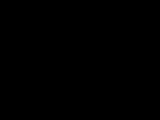
\includegraphics[width=30mm]{MovedObjectFD}&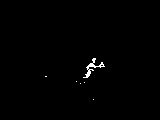
\includegraphics[width=30mm]{MovedObjectAM}\\
% \newline
% \parbox[top]{30mm}{Time of day} & 
\includegraphics[width=30mm]{TimeOfDay} & 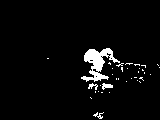
\includegraphics[width=30mm]{TimeOfDayFD}&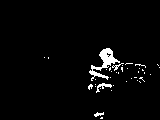
\includegraphics[width=30mm]{TimeOfDayAM}\\
% \newline
% \parbox[top]{30mm}{Light switch} & 
\includegraphics[width=30mm]{LightSwitch} & 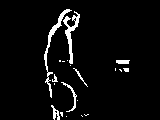
\includegraphics[width=30mm]{LightSwitchFD}&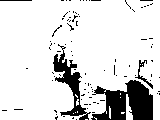
\includegraphics[width=30mm]{LightSwitchAM}\\
% \newline
% \parbox[top]{30mm}{Waving trees} & 
\includegraphics[width=30mm]{WavingTrees} & 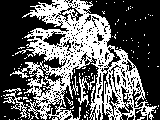
\includegraphics[width=30mm]{WT}&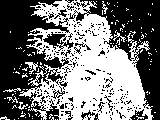
\includegraphics[width=30mm]{WavingTreesAM}\\
% \newline
% \parbox[top]{30mm}{Camouflage} & 
\includegraphics[width=30mm]{Camouflage} & 
\includegraphics[width=30mm]{CamouflageFD}&
\includegraphics[width=30mm]{CamouflageAM}\\
% \newline
% \parbox[top]{30mm}{Bootstrapping} & 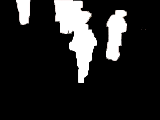
\includegraphics[width=30mm]{Bootstrapping} & 
\includegraphics[width=30mm]{BootstrappingFD}&
\includegraphics[width=30mm]{BootstrappingAM}\\
% \newline
% \parbox[top]{30mm}{Foreground aperture} & 
\includegraphics[width=30mm]{ForegroundAperture} & 
\includegraphics[width=30mm]{ForegroundApertureFD}&
\includegraphics[width=30mm]{ForegroundApertureAM}\\
% \end{tabular}
% \label{tab:gt}
% \end{table}

% \begin{table}[h!]
%   \centering
%   \footnotesize
%   \begin{tabular}[h]{c|ccc|ccc}
%      & Frame Difference  &  &  & Approximate Median &  & \\ 
%  & Precision & Recall & PCC & Precision & Recall & PCC\\ \hline
% Moved Object & - & - & 1 & - & - & 0.9942\\ 
% Time of Day & 0.7514 & 0.4048 & 0.9496 & 0.6573 & 0.2539 & 0.9392\\ 
% Light Switch & 0.6564 & 0.204 & 0.858 & 0.1282 & 0.6982 & 0.2057\\ 
% Waving Trees & 0.4508 & 0.5628 & 0.6571 & 0.5748 & 0.8795 & 0.7645\\ 
% Camouflage & 0.7463 & 0.0588 & 0.4736 & 0.9311 & 0.9418 & 0.9299\\ 
% Bootstrapping & 0.6504 & 0.3808 & 0.889 & 0.555 & 0.5787 & 0.8807\\ 
% Foreground Aperture & 0.6342 & 0.1563 & 0.7606 & 0.5425 & 0.5434 & 0.765\\ 
%   \end{tabular}
%   \caption{Precision, recall and PCC metrics for background subtraction algorithms}
%   \label{tab:wallflower}
% \end{table} 


% Table \ref{tab:wallflower} lists the precision, recall and PCC values as discussed in Section \ref{sec:quant-analys} for all algorithms on all seven Wallflower videos. The lowest PCC that we see is for AMF on the light switch video, which highlights that approximate median is a very slowly adapting algorithm. Although the evaluation frame is 13 frames after the change in illumination, the AMF still classes a large part of the frame as foreground incorrectly, giving a low precision rating in Table \ref{tab:wallflower} and therefore a low PCC overall. 

% The ground truth for moved object is entirely background so we can only use the PCC metric when comparing algorithms. The results show that frame difference is much faster to adapt then approximate median, as the frame difference successfully identifies the entire evaluation frame as background giving it a PCC of 1. Due to AMF's slow adaption, it still detects some foreground in the evaluation image, even though the chair was moved 100 frame previous to the evaluation frame. AMF's slow adaption rate can also seen in foreground aperture where is a large section of missing foreground (False Negatives), where the person was originally sleeping. After he has woken up and moved, the AMF algorithm still believes strongly that this portion of the frame is background.

% Throughout the tests FD successfully determines the outline of the foreground but struggles to correctly detect the interior pixels, a flaw discussed earlier in Section \ref{sec:frame-difference}. This is particularly evident in the videos Light Switch and Camouflage which is why these videos have very low recall values. 

% Only one ground truth frame has been compared for each video sequence, and so to improve on this, precision and recall values have been calculated and plotted for nine adjacent frames. These curves were calculated for two video sequences; Waving Trees and Camouflage. Figure \ref{fig:wtg} shows precision and recall values for both frame differencing and approximate median methods on the Waving Trees sequence and Figure \ref{fig:cg} shows the same metrics but for the Camouflage video.

% \begin{figure}[h!]
%   \centering
%   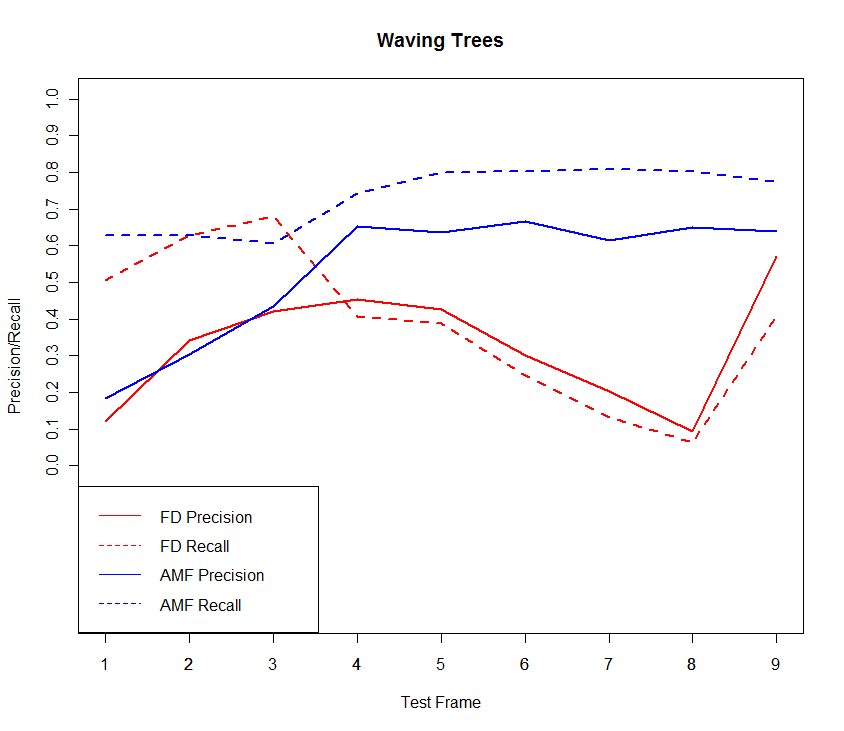
\includegraphics[width = 10cm]{wavingtreesgraph}
%   \caption{Precision and recall values for FD and AMF algorithms as implemented on the Waving Trees video.}
%   \label{fig:wtg}
% \end{figure}

% \begin{figure}[h!]
%   \centering
%   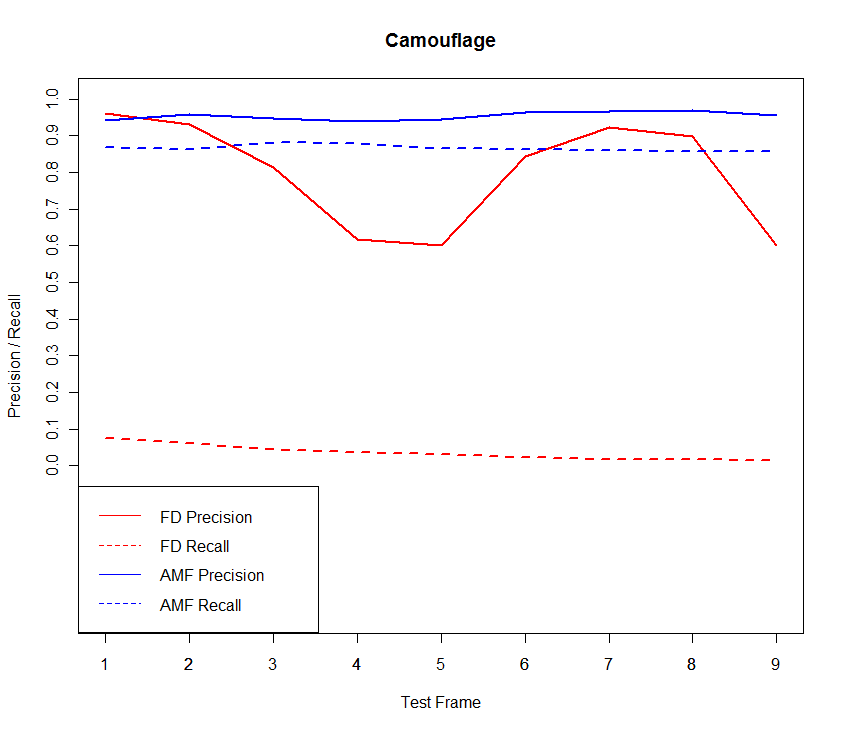
\includegraphics[width = 10cm]{camouflagegraph}
%   \caption{Precision and recall values for FD and AMF algorithms as implemented on the Waving Trees video.}
%   \label{fig:cg}
% \end{figure}

% We can see clearly in Figure \ref{fig:cg} that the recall values for the frame differencing method are consistently low, this is due to the aperture affect discussed earlier. Both metrics recall and precision are generally higher when using the approximate median filter than when the frame differencing method.

% Figure \ref{fig:wtg} also shows that approximate median method metrics are higher than those of the frame differencing. Both methods seem to suffer from low precision in the video and this can be explained by a failure of both algorithms to correctly identify the moving tree as background. 

% In general, frame differencing has performed poorly for most of the videos in this dataset, and has struggled particularly with recall as can be seen by the low values in Table \ref{tab:wallflower}. Approximate median filtering did perform better than frame differencing but still struggled on a number of videos, particularly in sequences featuring a highly dynamic background or rapid illumination. Better segmentation is required of background subtraction methods if these are to be implemented within surveillance systems. Real-life scenarios require video analysis systems which are capable of processing, storing and transmitting data collected by many high-definition cameras in real-time and under bandwidth constraints. 

% The next section discusses compressive sensing, an emerging topic in signal processing which offers a new way to approach this problem by reducing the amount of data collected by the surveillance system whilst retaining the ability to accurately represent the original signal. 


%Spare Notes

%CHEUNG: Slow adaption seems to work better than fast adaption becuase slow adaption prevents transient foreground from adapting the background but it struggles with start/stop changes.  GAP in research robustness against environmental noise, sudden change in illumination, achieveing the balance between fast adaptation and robust modelling. 

%\cite{maddalena2008self} differences in texchniques s, parametric vs non parametric. Para have to make assumptions which may not fit the data and choosing parameter can be cumbersome, non para are more flexible but heavily data dependent. Unimodal vs Multimodal, unimodal are low complexity but cant dealing with moving backgrounds such as EXAMPLE, multi are good but complex.  Considers five video sequences including waving trees and time of day from wallflower dataset.

%She claims that average filtering is not robust to scenes with many moving objects particulary if they move slowly. It cant handle bimodal backgrounds. one threshold for the whole sequence. all information fomr both bg and fg is used for background modelling. Slow moving objects will make the algorithm fail. Computational complexity and storage of MoG is linear in terms of the number of componenets K. Used the UCSD and wallflower datasets. She tested FD, AMF, GMM and ViBe on all 7 wallflower and looked at recall, precision and PCC. Video 1 , testing the adaption rate of algorithms. FD great, others ok. Vid 2 (gradual illuminaiton) Vibe and GMM good. FD and AMF fail to detect object. Vid 3. FD does best at outline but not whole object, AMF is bad, GMM middling. Vid 4 trees.FD not good, AMF and GMM are similar and ok. She hints that the multiple parameters make the optimnization of GMM difficult. Vid 5 camoflage. FD outline only,GMM not fast enough, AMF good performance. Vid 6 bootstrapping. non great, AMF the best. Vid 7, sleeping, GMM fails not fast enough, AMF best again. No real conclusion. Main limitations \cite{cheung2004robust}. Ignore correlation between neighbouring pixels, rate of adaption may not match moving speed of foreground, non stationary pixels from leaves or shadows as mistaken as true moving objects. most techniques work on one pixel at a time independently. Is this a good idea?


%---------------- COMMENT FOR IMPORTING ----------------------
%\pagebreak											%Comment for importing
%\bibliographystyle{plainnat}		%Comment for importing
%\bibliography{References}				%Comment for importing
%\end{document}									%Comment for importing
%-------------------------------------------------------------
